\part{Fault tolerance}
\section{Learning Goals:}
\begin{itemize}
    \item Understand/use: Reliability. Failure, fault, error. Failure Modes. Acceptance Test. Fault prevention vs. fault tolerance. Redundancy. Redundancy, static vs. dynamic. Forward/Backward error recovery
    \item Understand/use/evaluate techniques: N-version programming. Recovery blocks. Error detection. Failure mode merging. Acceptance tests 
\end{itemize}

\section{Reliability, Failure and faults}
There are 4 sources of faults in embedded systems
\begin{enumerate}
    \item Inadequate specification, i.e. misunderstanding the interactions between the program and the environment.
    \item Design errors in software components.
    \item Failure of hardware components. 
    \item Interference in the supporting communication subsystem.
\end{enumerate}

\textbf{Reliability} is a measure of the success with which the system conforms to some specification of its behavior. \textbf{Failure} is when the behavior of the system deviates from that which is specified for it. It in other words fail to follow specification. \textbf{Errors} are unexpected problems internal to the system which eventually manifests themselves in system's external behavior. \textbf{Faults} are the mechanical or software-related cause of failure. A failure in one (sub)system can cause faults in other systems:

\begin{figure}[H]
\centering
    Fault $\xrightarrow{\text{activation}}$ Error $\xrightarrow{\text{propagation}}$ Failure $\xrightarrow{\text{causation}}$ Fault
\end{figure}
Fault types
\begin{itemize}
\item Transient faults: Occur at some point in time, then disappear at some later point in time. E.g. hardware response to external electromagnetic field, fault disappears when the field disappears. Common kind of fault in communication systems.
\item Permanent faults: Occur at some point in time, lasts indefinitely until repair. E.g. software design faults.
\item Intermittent faults: Transient faults that sometimes happen and sometimes not. E.g. fault due to heat on heat sensitive hardware component.
\end{itemize}

Software faults are also called Bugs and we have two types:
\begin{itemize}
\item Bohrbugs: Reproducible, usually identifiable. Can be found and fixed with testing usually or diversity techniques.
\item Heisenbugs: Only activate under certain unknown, rare circumstances. Usually not found during testing. E.g. code shared between concurrent tasks that is not properly synchronized. Causes can be software ageing i.e. not freeing allocated memory. 
\end{itemize}

\subsection{Failure modes}
In short, failure modes describe the ways a (sub)system can fail.

We have two general classes of failure modes
\begin{itemize}
\item Value failure: Error in the value associated with service. Can be the result of a data conversion for example. The two categories are:
\begin{itemize}
    \item Constraint error: A fault causes a constraint to be breached.
    \item Value error: A fault causes a value to be incorrect.
\end{itemize}
\item Time failure: Service not delivered at the correct time. The thee categories are:
\begin{itemize}
    \item Too early
    \item Too late (Performance error)
    \item Infinitely late (Omission error)
\end{itemize}
\end{itemize}
Combination is called arbitrary failures. We also have \textbf{Commission/Impromptu} failure which describes a situation where a service delivered is not expected.

\begin{figure}[H]
\centering
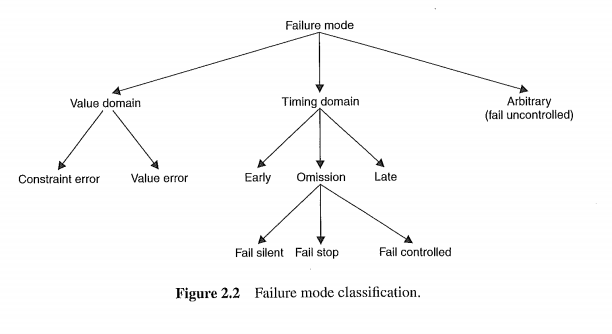
\includegraphics[width=0.5\textwidth]{figures/Fault_Tolerance/failure_mode_classification.PNG}
\end{figure}

Based on these failure modes we can sum up how the system might fail.
\begin{itemize}
\item Fail uncontrolled: Arbitrary or impromptu errors
\item Fail late: delivers service too late
\item Fail silent: Omission failure
\item Fail stop: Omission failure, but other systems can detect it.
\item Fail controlled: fails in a specified controlled manner.
\item Fail never: Self-explanatory.
\end{itemize}

\section{Fault prevention and fault tolerance}
\textbf{Fault prevention} aims to eliminate any and all faults before the system goes into operation, whilst \textbf{fault tolerance} enables the system to continue functioning even in the presence of faults. Both approaches attempt to give the system well-defined failure modes.

\subsection{Fault prevention}
Consists of two stages;
\begin{itemize}
\item Fault avoidance - Achieved by choosing reliable components, eliminating interference, having a complete requirements specification, following strict design methodologies and using languages with data abstraction and modularity, like Ada and Java.
\item Fault removal - Removing causes of errors mainly by system testing. Note that system testing is difficult. 
\end{itemize}
Any system will fail eventually either in hardware or software, and for real-time systems we therefore need fault tolerance.

\subsection{Fault tolerance}
Three levels of fault tolerance
\begin{enumerate}
\item \textbf{Full fault tolerance} - The system continues to operate in the presence of faults for a limited time period with no significant loss of functionality or performance. Required in most safety-critical systems in theory.
\item \textbf{Graceful degradation} - also known as fail soft. The system continues to operate in presence of errors, accepting a partial degradation of functionality or performance until recovery or repair. Safety-critical systems often settle for this type of fault tolerance in practice. Graceful degradation necessity for applications with high availability requirements.
\item \textbf{Fail safe} - The system maintains its integrity while accepting temporary halt in  its operation. In other words, it shuts down safely temporarily to allow for maintenance. 
\end{enumerate}

The goal of fault tolerance is to minimize redundancy while maximizing reliability subject to cost, size and power constraints of the system.

\begin{figure}[H]
\centering
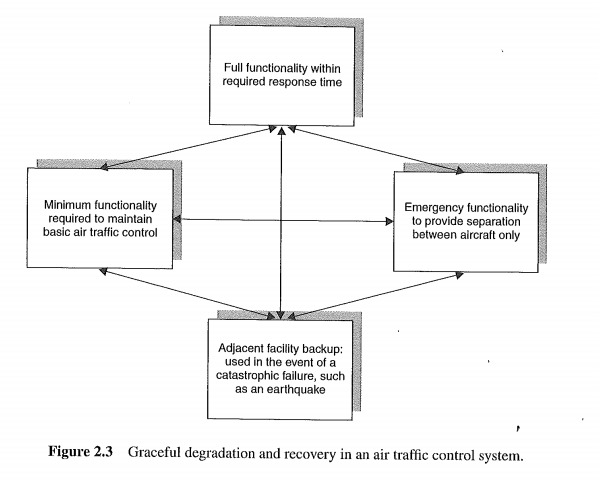
\includegraphics[width=0.5\textwidth]{figures/Fault_Tolerance/graceful_degradation_example.PNG}
\end{figure}

\subsection{Redundancy}
\textbf{Protective redundancy} introduces components that detects and recovers
the systems from faults, but are unnecessary for normal operation. When
designing a fault-tolerant system, the goal is to minimize redundancy while
maximizing reliability, subject to constraints on cost, size and power consumption. The redundant components can (and will) increase complexity, and it is useful to separate them from the rest of the system.
We separate between static and dynamic redundancy, both for hardware
and software. First, let’s have a look at hardware redundancy:

\begin{itemize}
\item Static redundancy (or masking) is based on redundant components
“hiding” faults. An example is Triple Modular Redundancy (TMR),
where a majority voting circuit is used. The output of three identical
components are compared, and if one differs from the others, its output
is masked out. It is assumed that faults are transient.
\item Dynamic redundancy is an error-detection facility within a component, making it possible for that component to indicate if its output is
in error. Note that the component does not hide or fix the error, that
must be done by some other part of the system. Examples are checksums (see parity byte section on Wikipedia for very simple example) and parity bits. 
\end{itemize}

For fault tolerance with regards to software design, we have \textit{N-version programming} which works like masking, and \textit{error detection and recovery}.
The latter is dynamic redundancy in the sense that recovery is only brought
into action once an error has occurred.

\section{N-version programming}
From one initial specification, N independent programs are created. In operation, they run concurrently, and their outputs are compared by a driver process. The “correct” result is determined by majority of vote, like with masking. 

Assumption: Program can be completely, consistently and unambiguously specified and independently developed programs will fail independently.

Example: On Boeing 777 flight control system, single Ada program was produced  but three different processors and three distinct compilers were used to obtain diversity.

The driver process invokes the versions, waits for completion of voting, compares results and acts on these results.

\begin{figure}[H]
\centering
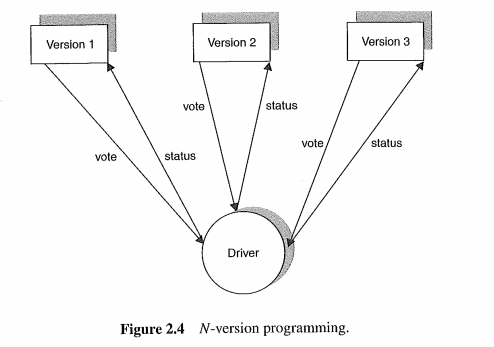
\includegraphics[width=0.5\textwidth]{figures/Fault_Tolerance/N_version_programming.PNG}
\end{figure}

In the context of embedded systems, we check the versions underway and not at the end. Interaction between the driver and the versions consists of 3 components
\begin{enumerate}
\item Comparison vectors: Also called votes, consists of output and metadata (attributes)
\item Comparison status indicators: Commands from driver. Indicates the actions that each version must perform as result of comparison. Can be \textit{continuation}, \textit{termination} or \textit{continuation with vote modification} on some of the versions.
\item Comparison points: The points in the code where votes must be communicated to the driver process.
\end{enumerate}

Challenges concerning N-version programming are:
\begin{itemize}
\item \textbf{Initial specification} - A specification error will manifest itself in all N versions of the implementation.
\item \textbf{Independence of design effort} - The assumption that versions will fail completely independently of each other is not reality in practice.
\item \textbf{Adequate budget} - N-version programming technique can require N times the budget of a 1 version technique.
\end{itemize}

\section{Software dynamic redundancy}
With dynamic redundancy, the redundant components only come into operation when an error manifests itself. There are four phases to dynamic redundancy in software:
\begin{enumerate}
\item \textbf{Error detection} - Most faults will manifest themselves in form of an error. No Fault tolerance scheme can be utilized until the error is detected.
\item \textbf{Error diagnosis} - There is a delay between a fault becoming active and error detection, the propagation of erroneous information in the system is assessed.
\item \textbf{Error recovery} - Transform the corrupted system into a state form which it can continue its normal operation (perhaps with degraded functionality).
\item \textbf{Fault treatment} - Maintenance must be performed to correct the underlying fault responsible for the error.

\end{enumerate}

\subsection{Error detection}
There are two classes:
\begin{itemize}
\item \textbf{Environmental detection} - Detection by hardware or run-time support system. E.g. overflow error in hardware or out-of-bounds error for array in run-time)
\item \textbf{Application detection} - Detect error with application specific code.
\begin{itemize}
    \item \textbf{Replication checks} - N-version programming with N=2
\item \textbf{Timing checks} - Watchdog or deadline checks
\item \textbf{Reversal checks} - Calculate input from output and check for match.
\item \textbf{Coding checks} - Test for corruption of data. Based on redundant data, i.e. checksum.
\item \textbf{Reasonableness checks} - Are based on knowledge of the internal design and construction of the system. I.e. range violation and assertions.
\item \textbf{Structural checks} - Metadata about structures
\end{itemize}
\end{itemize}
Note that all forms of application detection mentioned can be implemented in hardware and are then considered to be environmental detection.

\subsection{Error diagnosis}
Software designers aim to minimize the damage caused by a faulty component, this is called firewalling. Two techniques are:
\begin{itemize}
\item \textbf{Modular decomposition} - Modules only communicate through well defined interfaces, internal details are hidden. Provides a static structure.
\item \textbf{Atomic actions} - are indivisible, and appear to happen instantaneously for the rest of the system. Often called \textbf{transactions} or atomic transactions. They are used to move the system from one consistent state to another, and limit the flow of information between components/modules.
\end{itemize}

\subsection{Error recovery}
The two approaches here are forward and backward error recovery.
\begin{itemize}
\item \textbf{Forward Error Recovery} - Attempts to continue from the corrupted state by making selective corrections to the state.
\item \textbf{Backward Error Recovery} - Relies on restoring the system to a safe state previous to that in which the error occurred. This safe state is called an recovery point and the act of establishing it is called \textbf{checkpointing}.
\end{itemize}

Advantage of backward error recovery is that it does not rely on finding the location or cause of faults. Can therefore be used to recover from unanticipated faults including design errors. A disadvantage on the other hand is that it cannot undo effects the fault may have had on the environments (missile launch) and it can be time-consuming. Another disadvantage is the possibility of the domino effect.

\textbf{The domino effect} is a possible issue in state restoration with concurrent processes. Consider the following scenario in Figure \ref{fig: domino_effect}. 

\begin{figure}[H]
\centering
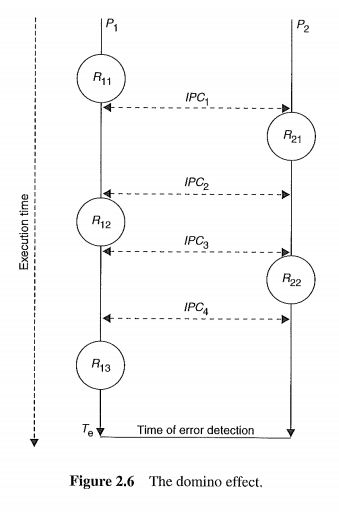
\includegraphics[width=0.5\textwidth]{figures/Fault_Tolerance/domino_effect.PNG}
\label{fig: domino_effect}
\end{figure}

If P1 detects an error at Te then it is simply rolled back to R13. If on the other hand P2 detects an error at Te it is rolled back to R22 and thus must undo IPC4. This means that P1 must be rolled back to R12 which means it must undo IPC3 which means P2 must rollback to R21 and undo IPC2 and so on. Potentially the two processes have to be rolled back to the beginning of their interaction. The only way to be guaranteed to stop this is with \textbf{recovery lines} which are consistent set of recovery points across all processes that communicates together.

\section{Recovery blocks and acceptance tests}
Recovery blocks are normal blocks in the programming language sense but where the entrance is an automatic recovery point and the exit an acceptance test. 
\begin{figure}[H]
\centering
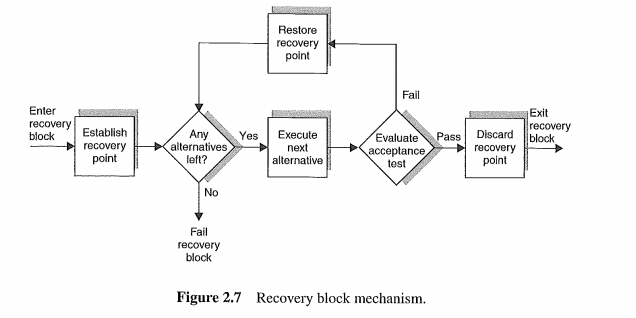
\includegraphics[width=\textwidth]{figures/Fault_Tolerance/recovery_block_mechanism.PNG}
\end{figure}

\subsection{Acceptance test}
The acceptance test is used to test that system is in an acceptable state after the execution of the block (also called primary module). If it fails program is restored to recovery point at beginning of block and an alternative module is being executed. If all alternative modules fail the block fails.

One should keep in mind the tradeoff between comprehensive testing and keeping overhead at a minimum. All error detection techniques mentioned earlier may be used as acceptance tests.

\subsection{Comparison between N-version programming and recovery blocks}
\begin{itemize}
\item \textbf{Static vs. Dynamic}-version is static because all versions run all the time. Recovery blocks are dynamic because the alternative code only runs when acceptance test fails.
\item \textbf{Associated overhead} - Both methods increase overhead/complexity.
\item \textbf{Diversity of design} - Both exploit this and are therefore susceptible to errors that originate in the specification.
\item \textbf{Error detection} - N-version uses vote and recovery blocks uses acceptance test. Exact voting less overhead than acceptance testing. Same cannot be concluded for inexact voting.
\item \textbf{Atomicity} - Backward error recovery criticized because cannot undo effects or damage which may have occurred in the environment. N-version programming avoids this because all versions are assumed to not interfere with each other; they are atomic. They communicate only with the driver through voting. Not that it is possible to structure program such that unrecoverable operations do not occur in recovery blocks.

Note that N-version programming and recovery blocks can be considered competing techniques, but also complementary techniques.
\end{itemize}

\section{Dynamic redundancy and exceptions}


The goal if this section is to introduce framework for implementing software fault tolerance based on dynamic redundancy and the notion of exceptions and exception handlers.

An \textbf{exception} is the occurrence of an error. \textbf{Raising} (or throwing or signaling) an exception is bringing the exception condition to the attention of the invoker of the operation which caused the exception. In less formal wording, this means letting the program know an error has occurred. \textbf{Handling} (or catching) an exception is the invoker's response to the raised exception.

Note that exception handling is a forward error recovery mechanism, but it can also be used to provide backward error recovery.

\begin{figure}[H]
\centering
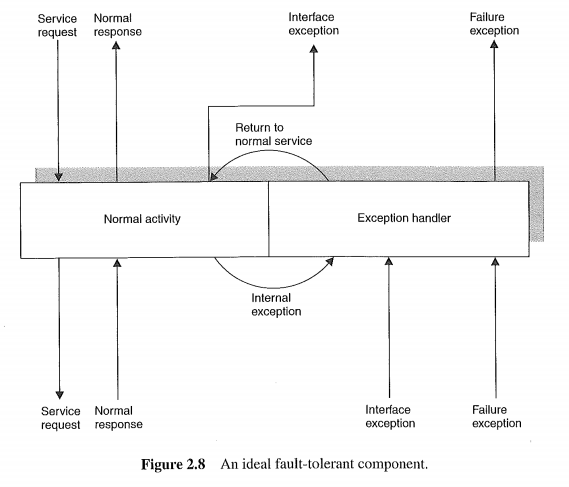
\includegraphics[width=\textwidth]{figures/Fault_Tolerance/ideal-fault-tolerant-component.PNG}
\end{figure}



